% !TEX root = main.tex
%%%%%%%%%%%%%%%%%%%%%%%%%%%%%%%%%%%%%%%%%%%%%%%%%%%%%%%%%%%%%%%%%%%%%%%%%%%%%%%%
% Survival Analysis
%%%%%%%%%%%%%%%%%%%%%%%%%%%%%%%%%%%%%%%%%%%%%%%%%%%%%%%%%%%%%%%%%%%%%%%%%%%%%%%%
\section{Survival Analysis}
\label{section:survival}

 Kaplan-Meier survival analysis (KM) gives the probability of survival
beyond a given time. It is a nonparametric technique that makes no
specific failure model assumptions, such as Weibull, Exponential,
etc. It can also split the data into subpopulations and compute
separate survival curves. 

If $T$ is taken to be the random variable of a GPU fail time, then its
probability density function is $f(t)$ and its cumulative distribution
function $F(t) = Pr\{T < t\}$ gives the probability that a GPU fails
by duration $t$. The survival function is then 
\begin{displaymath}
  S(t) = Pr\{T \geq t\} = 1 - F(t) = \int_t^\infty f(x)dx,
\end{displaymath}
which is the probability of being operational at duration
$t$.

We use reliability censoring concepts to use information from units
that were proactively removed before failing as well as those still in
operation till the end. We use the R package {\tt survival} for the KM
analysis.
\begin{figure*}
  \centering
  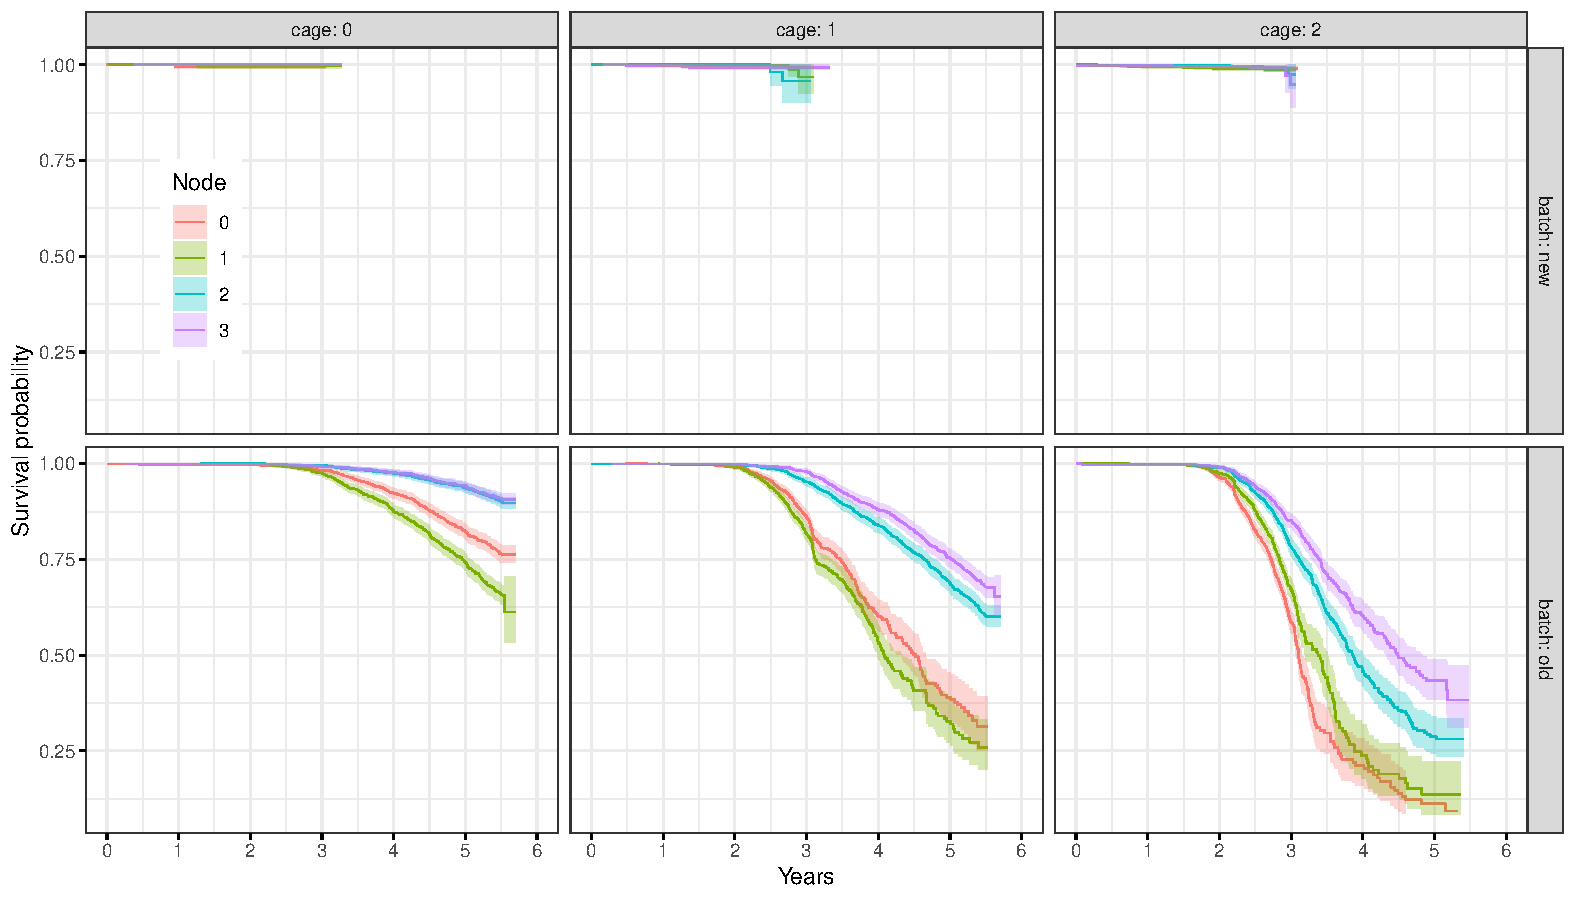
\includegraphics[width=7in]{figs/km_cage-node_a001.pdf}
  \caption{Comparison of the old and new batches, including survival
    differences based on {\tt cage} and {\tt node} GPU locations.}
  \label{fig:km-all-cage-node}
\end{figure*}

A sister concept to the survival function is the hazard function:
\begin{displaymath}
  H(t) = \frac{f(t)}{S(t)},
\end{displaymath}
which is what is sometimes called the "bathtub" curve in reliability.


The Cox proportional hazards (CPH) regression analys
\cite{Cox1972,Harrell2015} takes the hazard function above and a set
of covariates $x$ and models $k$s GPU hazard as 
\begin{displaymath}
  H_k(t) = H_0(t)e^{\sum\limits_{i=1}^n{\beta x}}
\end{displaymath}
That is, a base hazard rate multiplied by a function of
covariates. The key assumption in the CPH model is that the "hazards"
are multipliers on the "baseline hazard" but the estimate of the
baseline hazard is nonparametric, meaning it makes no specific
distributional assumption and just learns from the data (unlike
analyses that assume for example a Weibul or an exponential
model). The multiplicative assumption is that the hazard curves do not
cross and are multiples of each other. The multiplier is the *hazard
coefficient*. For example, if the baseline is *node0* and the *node2*
hazard is 2, then *node2* sees twice as many failures as *node0* on
average. 

For our comparison of hazards, we use as *covariates* all the unpacked
location variables, indicators whether the GPU has been moved, and our
notion of old and new GPUs based on first install date. Since many
GPUs experience time at more than one location, we use the longest
period location in this analysis. 

First, we do a univariate analysis for each covariate separately and
then we look at a multivariate view of this. Having multiple
covariates is called "multiple regression" as opposed to "multivariate
regression" reserved for cases with several response variables. The
univariate view is comparable to what would one see in a simple time
between failures analysis for a given population split. It can be
affected by sampling differences for other covariates. For example, if
the strongest effect is seen in a variable not used in a split and its
values are unevenly distributed across the split, its effect can leak
into the split. This is why we also do a multivariate analysis, where
the effect of each covariate is adjusted for all the other
covariates. 
 

\begin{figure}
  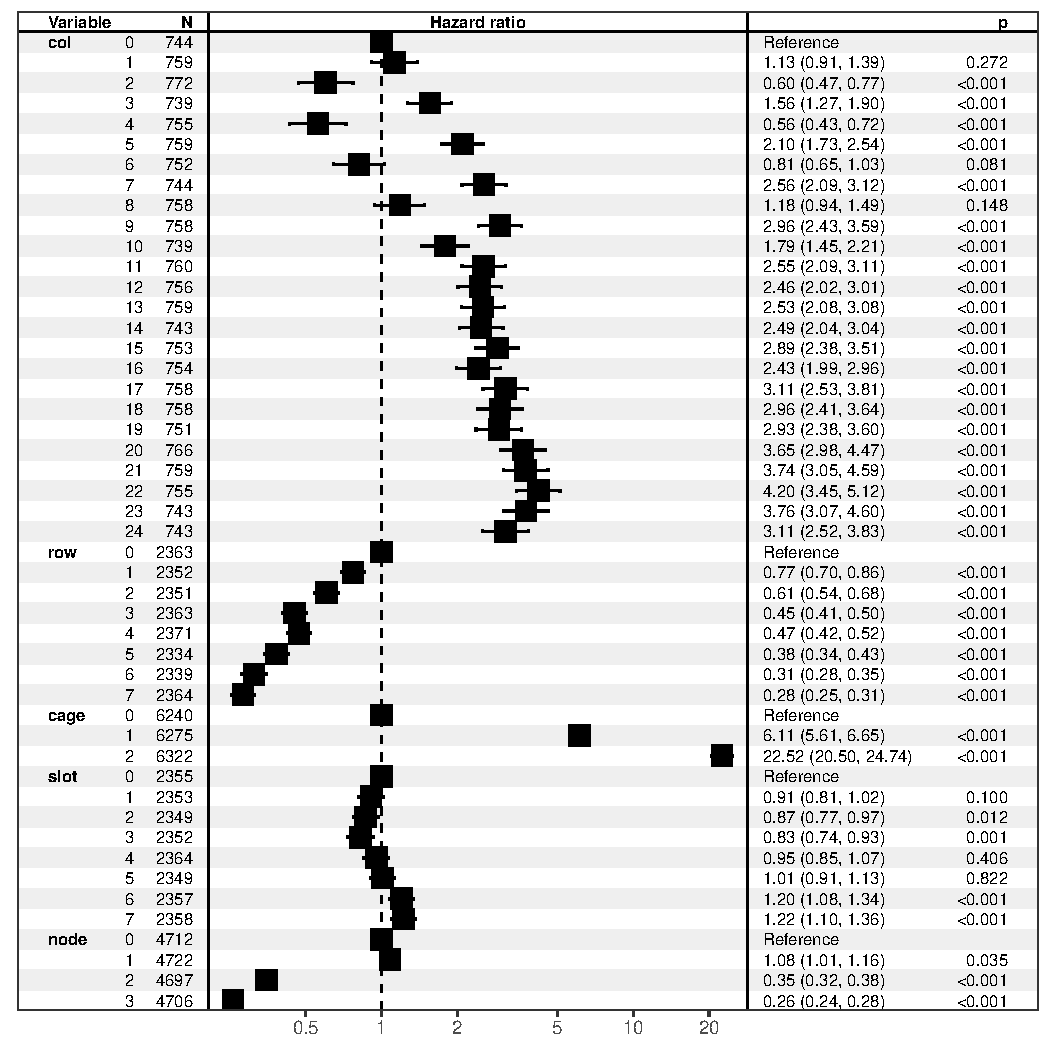
\includegraphics[width=\columnwidth]{figs/cox_o001.pdf}
  \caption{GPU hazard ratios from Cox regression model on {\tt old}
    batch.}
\end{figure}
\begin{figure}
  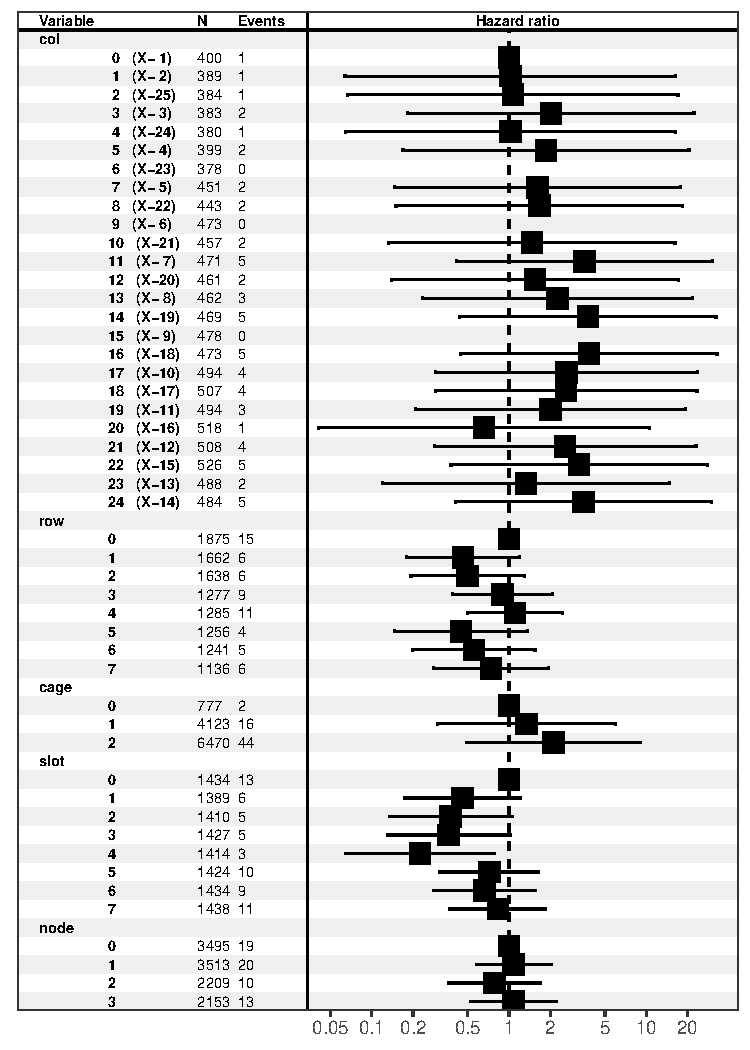
\includegraphics[width=\columnwidth]{figs/cox_n001.pdf}
  \caption{GPU hazard ratios from Cox regression model on {\tt new}
    batch.}
\end{figure}

Higher numbered columns appear to have a higher (up to about 2x)
failure rate. There actually seems to be a hint of three groups that
have similar rates: 0-6 baseline, 7-16 are 1.5x baseline, and 17-24
are 2x baseline. 

Higher numbered rows tend to have a lower (up to about 0.5x) failure rate.

This seems surprisingly strong! Higher numbered cages have failure
rates 5x and 16x higher than cage = 0. In fact, this seems so strong
that its effect could be leaking into all other comparisons under
uneven sampling!

Not much difference between slots. They are all close to the baseline
slot0.

Interestingly, nodes 2 and 3 have half the failure rate of nodes 0 and
1. Is this related to the cage variable or is there a real location
effect?

Now the multivariate Cox regression analysis, where each factor is
adjusted for all the other factors. This can fix some uneven sampling
and multivariate dependence. 

The col groups persist and are even stronger. The row effect is also
stronger. The cage effect is out of this world! slot is still without
any effect. node effect also persists and is a bit stronger. 

Let’s separate the “old” and “new” batches of GPUs and run separate
Cox models. 
